\section{Relations between OT Security Notions}


\begin{figure}[h!]
\centering
\begin{tikzpicture}
\node (U) at (4,4) {Uniform Security};
\node (SC) at (0,2) {Sender Tweakable};
\node (RC) at (8,2) {Receiver Tweakable};
\node (E) at (4,0) {Endemic Security};
\node (TC) at (3,2) {Coin Tossing};
\draw [-implies,double equal sign distance] (U) -- (SC);
\draw [-implies,double equal sign distance] (U) -- (RC);
\draw [-implies,double equal sign distance] (SC) -- (E);
\draw [-implies,double equal sign distance] (RC) -- (E);
\draw [->, thick] (U) to [out=240,in=90] (TC);
\draw [-, thick] (E) to [out=60,in=270] (5,2);
\draw [->, thick] (5,2) to [out=90,in=300] (U);
\draw [-, thick] (TC) to [out=0,in=300] (4.655,3);
\draw [->, thick] (E) to [out=180,in=270] (SC);
\draw [->, thick] (E) to [out=0,in=270] (RC);
\end{tikzpicture}
\label{fig:OTrelations}
\caption{
The figure depicts the different security notions of OT and their relations. $A\Rightarrow B$ denotes that security $A$ implies security $B$. $A\rightarrow B$ denotes that any OT realizing security $A$ can be efficiently transformed into an OT realizing security $B$.
}
\end{figure}

\begin{lemma}\label{lemma:is_a}
Let the distribution of OT strings be efficiently sampleable. 
Then a uniform security implies sender as well as a receiver tweakable security. If \OT is a sender or receiver tweakable secure, then it is also an endemically secure.
\end{lemma}

\begin{proof}
In the first step, we show that uniform security implies sender tweakable security and receiver tweakable security implies endemic security. These two implications result from the same simple fact that a malicious sender interacting with the ideal OT is easier to construct when it can choose the OT strings rather than if it receives the strings from the ideal OT. The following claim formalizes this fact. 
\begin{claim}\label{claim:utocs}
Let \OT be secure against a malicious sender with respect to an ideal OT $\OOT^*$ that sends the OT strings $(s_i)_{i\in[n]}$ to the sender, i.e. oracle $\OOT^u$ and $\OOT^{\rec}$, and the distribution of $(s_i)_{i\in[n]}$ is efficiently sampleable. Then \OT is also secure against a malicious sender with respect to ideal OT $\OOT^{\send}$, which receives the OT strings $(s_i)_{i\in[n]}$ from the sender.
\end{claim}


\begin{proof}
We show that if there is an adversary that breaks the security against a malicious security with respect to ideal OT $\OOT^{\send}$ then there is also an adversary that breaks the security with respect to $\OOT'$. More precisely, if there is a ppt adversary $\Adv_1$ such that for any ppt adversary $\Adv_1'$ there exists a ppt distinguisher $\D_1$ with 
$$
|\Pr[\D_1((\Adv_1,\rec)_{\langle \Adv_1, \rec\rangle})=1] -\Pr[\D_1( (\Adv'_1, \O_{\OT, \rec}^{\send})_{\langle \Adv_1', \OOT^{\send}\rangle})=1]|=\epsilon,
$$
where $\O_{\OT, \rec}^{\send}$ is the \rec's side output within the view of $\OOT^{\send}$ and all algorithms receive input $1^\sec$. \rec additionally receives input \set.
Then there is also a ppt adversary $\Adv_2$ such that for any ppt adversary $\Adv_2'$ there exists a ppt distinguisher $\D_2$ with 
$$
|\Pr[\D_2((\Adv_2,\rec)_{\langle \Adv_2, \rec\rangle})=1] -\Pr[\D_1( (\Adv'_2, \O_{\OT, \rec}^*)_{\langle \Adv_2', \OOT^*\rangle})=1]|=\epsilon,
$$
where $\O_{\OT, \rec}^*$ is the \rec's side output within the view of $\OOT^*$ and all algorithms receive input $1^\sec$. \rec additionally receives input \set.

We set $\Adv_2:=\Adv_1$ and $\D_2:=\D_1$. Further, for any $\Adv_2'$, there is an $\Adv_1'$  such that the distribution of $(\Adv'_2, \O_{\OT, \rec}^*)_{\langle \Adv_2', \OOT^*\rangle}$ is identical with the distribution $(\Adv'_1, \O_{\OT, \rec}^{\send})_{\langle \Adv_1', \OOT^{\send}\rangle}$. This follows from the fact that  $\Adv_1'$ could choose the OT strings $(s_i)_{i\in[n]}$  from the same distribution as $\OOT^*$ does and otherwise follow the description of $\Adv_2'$. Since $\D_1$ is successful for any $\Adv_1'$ it will be also for any $\Adv_2'$, which can be seen as a special case on over the set of all ppt adversaries $\Adv_1'$.
\end{proof}

The remaining two implications, from uniform security to receiver tweakable security and from sender tweakable security to endemic security follow in a similar fashion. Again it is easier to construct a malicious receiver interacting with the ideal OT when he can choose the OT strings rather than receiving them from the ideal OT.
\begin{claim}\label{claim:utocr}
Let \OT be secure against a malicious receiver with respect to an ideal OT $\OOT^*$ that sends the learned OT strings $(s_i)_{i\in\set}$ to the receiver, i.e. oracle $\OOT^u$ and $\OOT^{\send}$, and the distribution of $(s_i)_{i\in\set}$ is efficiently sampleable. Then \OT is also secure against a malicious sender with respect to ideal OT $\OOT^{\rec}$, which receives the OT strings $(s_i)_{i\in\set}$ from the receiver.
\end{claim}

\begin{proof}
The proof is basically identical to the proof of Claim~\ref{claim:utocs}. Again, the set of all ppt $\Adv_2'$ is a subset of the set of all ppt $\Adv_1'$ and identical with the set of all $\Adv_1'$ that sample  $(s_i)_{i\in\set}$ from the same distribution as when sent by $\OOT^*$.
\end{proof}

\end{proof}








\paragraph{Transformations.} 


\begin{figure}[t]
\centering
\framebox{
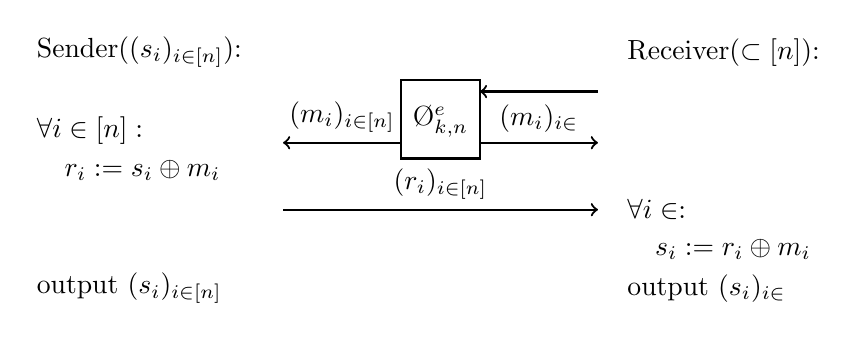
\begin{tikzpicture}
\node [anchor=west] at (0,5) {Sender$((s_i)_{i\in[n]})$:};
\node [anchor=west] at (7.5,5) {Receiver$(\set\subset[n])$:};
\draw [thick, <-] (5.75,4.5)-- node [midway,above]{$\set$}(7.25,4.5);
\draw [thick] (4.75,4.65)--(5.75,4.65)--(5.75,3.65)--(4.75,3.65)--cycle;
\node at (5.25,4.125){$\O^{e}_{k,n}$};
\node [anchor=west] at (0,4){$\forall i\in[n]:$};
\node [anchor=west] at (0,3.5){$\quad r_i:=s_i\oplus m_i$};

\draw [thick, ->] (3.25,3)-- node [midway,above]{$(r_i)_{i\in[n]}$}(7.25,3);
\node [anchor=west] at (7.5,3){$\forall i\in\set:$};
\node [anchor=west] at (7.5,2.5){$\quad s_i:=r_i\oplus m_i$};
\draw [thick, ->] (5.75,3.85)-- node [midway,above]{$(m_i)_{i\in \set}$}(7.25,3.85);
\draw [thick, <-] (3.25,3.85)-- node [midway,above]{$(m_i)_{i\in [n]}$}(4.75,3.85);
\node [anchor=west] at (0,2) {output $(s_i)_{i\in[n]}$};
\node [anchor=west] at (7.5,2) {output $(s_i)_{i\in\set}$};
\end{tikzpicture}
}
% 	\framebox{\begin{minipage}{0.95\linewidth}
% 			Input: The sender $\send$ has input $s_1,...,s_n\in \{0,1\}^\ell$ while the receiver $\rec$ has input $\set\subseteq [n]$ of size $k$.
% 			\begin{enumerate}
% 				\item \label{step:senderChosen_step1} The parties invoke $\O^{e}_{k,n}$ where $\rec$ takes the role of the receiver with inputs $\set$. $\send$ obtains $(m_i)_{i\in[n]}$ and $\rec$ obtains  from  $\O^{e}_{k,n}$. 
% 				\item \label{step:senderChosen_step2}  $\send$ sends the strings $r_1,...,r_n$ to $\rec$ where $r_i:=s_i\oplus m_i$.
% 				\item \label{step:senderChosen_step3}  $\rec$ outputs $(s_i)_{i\in \set}$ where $s_i:=m_i\oplus r_i$.
% 	\end{enumerate}\end{minipage}}
	\caption{Sender Chosen OT Protocol $\Pi^{\send}_{k,n}$ in the $\O^{e}_{k,n}$ hybrid (\definitionref{def:ot}). For all $i\in[n]$, $r_i$, $m_i$ and $s_i$ are in $\bits^\ell$.}
	\label{fig:protoSendOT}
\end{figure}


\begin{lemma}
	$\Pi^{\send}_{k,n}$ of \figureref{fig:protoSendOT} realizes the Sender Chosen Ideal OT $\OOT^{\send}$ (\definitionref{def:ot}) with unconditional security in the $\O^{e}_{k,n}$ hybrid.
\end{lemma}

\begin{proof}
	First let us consider any corrupt sender $\Adv_1$. We construct a new adversary $\Adv_1'$ which interacts with the oracle $\O^{\send}_{k,n}$ and produces an identical output  to $\Adv_1$.  $\Adv_1'$ plays the role of $\O^{e}_{k,n}$ and $\rec$ in $\Pi^{\send}_{k,n}$ while running $\Adv_1$. $\Adv_1'$ receives the endemic OT strings $m_1,...,m_n$ from $\Adv_1$%in \stepref{step:senderChosen_step1}
, along with the strings $r_1,...,r_n$% in \stepref{step:senderChosen_step2}
.  $\Adv_1'$ extracts the OT strings of $\Adv_1$ as $s_i:=r_i\oplus m_i$. $\Adv_1'$ sends $(s_i)_{i\in [n]}$ to $\O^{\send}_{k,n}$ and outputs whatever $\Adv_1$ outputs.
	
	Observe that the output of the honest receiver is identical when $\Adv_1$ interacts with $\rec$ in $\Pi^{\send}_{k,n}$ and when $\Adv_1'$ interacts with $\O^{\send}_{k,n}$.
	
	
	Now let us consider a corrupt receiver $\Adv_2$. We construct a new adversary $\Adv_2'$ which interacts with the oracle $\O^{\send}_{k,n}$ and produces an identical output distribution to $\Adv_2$. $\Adv_2'$ plays the role of $\O^{e}_{k,n}$ and $\send$ in $\Pi^{\send}_{k,n}$ while running $\Adv_2$. $\Adv_2'$ receives the set $\set\subset[n]$ of size $k$ and the endemic OT strings $(m_i)_{i\in \set}$ from $\Adv_2$% in \stepref{step:senderChosen_step1}
. $\Adv_2'$ sends $\set$ to  $\O^{\send}_{k,n}$ and receives $(s_i)_{i\in \set}$ in response. $\Adv_2'$ computes $r_i:=s_i\oplus m_i$ for $i\in \set$ and uniformly samples $r_i\gets \{0,1\}^\ell$ for $i\in [n]\setminus \set$. $\Adv_2'$ sends $r_1,...,r_n$ to $\Adv_2$ and outputs whatever $\Adv_2$ outputs.

	The transcripts of $\Adv_2$ in these two interactions are identical except for $(r_i)_{i\in [n]\setminus \set}$. Observer that in the real interaction for $i\in [n]\setminus\set$, $r_i:=s_i\oplus m_i$ where $m_i$ is sampled uniformly at random  by the oracle $\O^{e}_{k,n}$ and is independent of the transcript of $\Adv_2$ (conditioned on $r_i$). Therefore sampling $r_i$ directly induces an identical distribution. 
	
	Therefore, any distinguishing advantage $\Adv_1$ or $\Adv_2$ produces in protocol $\Pi^{\send}_{k,n}$ implies that $\Adv_1'$ or $\Adv_2'$ would produce the same advantage against the instantiation of $\O^{e}_{k,n}$, i.e. $\negl$.
\end{proof}


\begin{figure}[t]
\centering
\framebox{
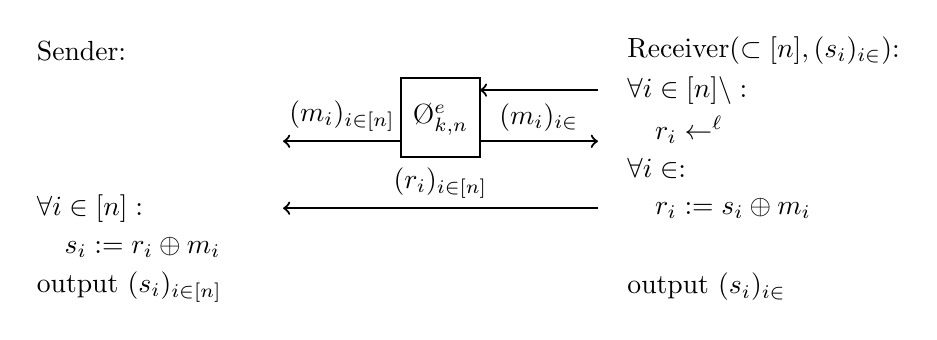
\begin{tikzpicture}
\node [anchor=west] at (0,5) {Sender:};
\draw [thick, <-] (5.75,4.5)-- node [midway,above]{$\set$}(7.25,4.5);
\node [anchor=west] at (7.5,5) {Receiver$(\set\subset[n],(s_i)_{i\in\set})$:};
\draw [thick] (4.75,4.65)--(5.75,4.65)--(5.75,3.65)--(4.75,3.65)--cycle;
\node at (5.25,4.125){$\O^{e}_{k,n}$};
\node [anchor=west] at (0,3){$\forall i\in[n]:$};
\node [anchor=west] at (0,2.5){$\quad s_i:=r_i\oplus m_i$};

\draw [thick, <-] (3.25,3)-- node [midway,above]{$(r_i)_{i\in[n]}$}(7.25,3);
\node [anchor=west] at (7.5,4.5){$\forall i\in[n]\setminus\set:$};
\node [anchor=west] at (7.5,4){$\quad r_i\leftarrow\bits^\ell$};
\node [anchor=west] at (7.5,3.5){$\forall i\in\set:$};
\node [anchor=west] at (7.5,3){$\quad r_i:=s_i\oplus m_i$};
\draw [thick, ->] (5.75,3.85)-- node [midway,above]{$(m_i)_{i\in \set}$}(7.25,3.85);
\draw [thick, <-] (3.25,3.85)-- node [midway,above]{$(m_i)_{i\in [n]}$}(4.75,3.85);
\node [anchor=west] at (0,2) {output $(s_i)_{i\in[n]}$};
\node [anchor=west] at (7.5,2) {output $(s_i)_{i\in\set}$};
\end{tikzpicture}
}
% 	\framebox{\begin{minipage}{0.95\linewidth}
% 			Input: The sender $\send$ has no input while the receiver $\rec$ has input $\set\subseteq [n]$ of size $k$ and $(s_i)_{i\in \set}$ where $s_i\in \{0,1\}^\ell$.
% 			\begin{enumerate}
% 				\item \label{step:receiverChosen_step1} The parties invoke $\O^{e}_{k,n}$ where $\rec$ takes the role of the receiver with inputs $\set$. $\send$ obtains $(m_i)_{i\in[n]}$ and $\rec$ obtains $(m_i)_{i\in \set}$ from  $\O^{e}_{k,n}$. 
% 				\item \label{step:receiverChosen_step2}  $\rec$ sends the strings $r_1,...,r_n$ to $\send$ where $r_i:=s_i\oplus m_i$ for $i\in \set$ and $r_i\gets\{0,1\}^\ell$ for $i\in [n]\setminus\set$.
% 				\item \label{step:receiverChosen_step3}  $\send$ outputs $(s_i)_{i\in [n]}$ where $s_i:=m_i\oplus r_i$.
% 	\end{enumerate}\end{minipage}}
	\caption{Receiver Chosen OT Protocol $\Pi^{\rec}_{k,n}$ in the $\O^{e}_{k,n}$ hybrid (\definitionref{def:ot}). For all $i\in[n]$, $r_i$, $m_i$ and $s_i$ are in $\bits^\ell$.}
	\label{fig:protoRecvOT}
\end{figure}


\begin{lemma}
	$\Pi^{\rec}_{k,n}$ of \figureref{fig:protoRecvOT} realizes the Receiver Chosen Ideal OT $\OOT^{\rec}$ (\definitionref{def:ot}) with unconditional security in the $\O^{e}_{k,n}$ hybrid.
\end{lemma}

\begin{proof}
	First let us consider any corrupt sender $\Adv_1$. We construct a new adversary $\Adv_1'$ which interacts with the oracle $\O^{\rec}_{k,n}$ and produces an identical output distribution as $\Adv_1$.  $\Adv_1'$ plays the role of $\O^{e}_{k,n}$ and $\rec$ in $\Pi^{\rec}_{k,n}$ while running $\Adv_1$. $\Adv_1'$ receives the endemic OT strings $m_1,...,m_n$ from $\Adv_1$% in \stepref{step:receiverChosen_step1}
. $\Adv_1'$ invokes $\O^{\rec}_{k,n}$ as the sender and receives $s_1,...,s_n$ in response. $\Adv_1'$ sends $r_1,...,r_n$ to $\Adv_1$ where $r_i:=m_1\oplus s_i$ and 	 outputs whatever $\Adv_1$ outputs.
	
	The transcripts of $\Adv_1$ in these two interactions are identical except for $(r_i)_{i\in [n]\setminus \set}$. Observer that in the real interaction for $i\in [n]\setminus\set$, $r_i\gets\{0,1\}^\ell$ while $\Adv_1'$ chooses $r_i:=m_1\oplus s_i$ where $s_i$ is sampled uniformly at random by $\O^{\rec}_{k,n}$. Therefore computing $r_i:=m_1\oplus s_i$ is identically distributed to $r_i\gets\{0,1\}^\ell$ given that $s_i\gets\{0,1\}^\ell$ is independent of the transcript of $\Adv_1$. 
	
	
	Now let us consider a corrupt receiver $\Adv_2$. We construct a new adversary $\Adv_2'$ which interacts with the oracle $\O^{\rec}_{k,n}$ and produces an identical output as $\Adv_2$. $\Adv_2'$ plays the role of $\O^{e}_{k,n}$ and $\send$ in $\Pi^{\rec}_{k,n}$ while running $\Adv_2$. $\Adv_2'$ receives the set $\set\subset[n]$ of size $k$ and the endemic OT strings $(m_i)_{i\in \set}$ from $\Adv_2$% in \stepref{step:receiverChosen_step1}
. $\Adv_2'$ receives $r_1,...,r_n$ from $\Adv_2$% in \stepref{step:receiverChosen_step2} 
 and extracts $(s_i)_{i\in \set}$ as $s_i:=r_i\oplus m_i$. $\Adv_2'$ sends $\set$ and $(s_i)_{i\in \set}$ to $\O^{\rec}_{k,n}$ and outputs whatever $\Adv_2$ outputs.
	
	The output distribution of he honest sender is identical in these two interactions is identical except for $(s_i)_{i\in [n]\setminus \set}$. In the real interaction \send outputs $s_i:=m_i\oplus r_i$ where $m_i$ is sampled uniformly by $\O^{e}_{k,n}$ and independent of the transcript. Therefore $\O^{\rec}_{k,n}$ sampling $s_i\gets\{0,1\}^\ell$ directly is identically distributed.
	
	Therefore, any distinguishing advantage adversary $\Adv_1$ or $\Adv_2$ produces in protocol $\Pi^{\rec}_{k,n}$ implies  that $\Adv_1'$ or $\Adv_2'$ would produce the same advantage against the instantiation of $\O^{e}_{k,n}$, i.e. $\negl$.
\end{proof}



\begin{figure}[t]
\centering
\framebox{
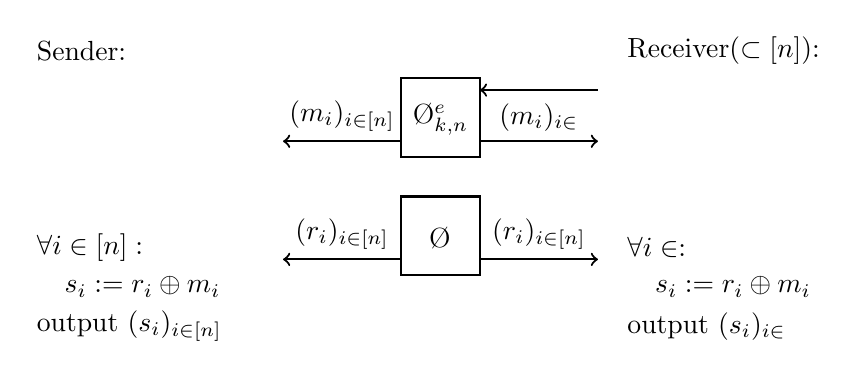
\begin{tikzpicture}
\node [anchor=west] at (0,5) {Sender:};
\node [anchor=west] at (7.5,5) {Receiver$(\set\subset[n])$:};
\draw [thick, <-] (5.75,4.5)-- node [midway,above]{$\set$}(7.25,4.5);
\draw [thick] (4.75,4.65)--(5.75,4.65)--(5.75,3.65)--(4.75,3.65)--cycle;
\node at (5.25,4.125){$\O^{e}_{k,n}$};
\draw [thick, ->] (5.75,3.85)-- node [midway,above]{$(m_i)_{i\in \set}$}(7.25,3.85);
\draw [thick, <-] (3.25,3.85)-- node [midway,above]{$(m_i)_{i\in [n]}$}(4.75,3.85);
\draw [thick] (4.75,3.15)--(5.75,3.15)--(5.75,2.15)--(4.75,2.15)--cycle;
\node at (5.25,2.625){$\O^{\coin}$};
\draw [thick, ->] (5.75,2.35)-- node [midway,above]{$(r_i)_{i\in [n]}$}(7.25,2.35);
\draw [thick, <-] (3.25,2.35)-- node [midway,above]{$(r_i)_{i\in [n]}$}(4.75,2.35);

\node [anchor=west] at (0,2.5){$\forall i\in[n]:$};
\node [anchor=west] at (0,2){$\quad s_i:=r_i\oplus m_i$};
\node [anchor=west] at (7.5,2.5){$\forall i\in\set:$};
\node [anchor=west] at (7.5,2){$\quad s_i:=r_i\oplus m_i$};

\node [anchor=west] at (0,1.5) {output $(s_i)_{i\in[n]}$};
\node [anchor=west] at (7.5,1.5) {output $(s_i)_{i\in\set}$};
\end{tikzpicture}
}
% 	\framebox{\begin{minipage}{0.95\linewidth}
% 			Input: The sender \send has no input and the  receiver \rec has input $\set\subseteq [n]$ of size $k$.
% 			\begin{enumerate}
% 				\item \label{step:uniform_step1} The parties invoke $\O^{e}_{k,n}$ where $\rec$ takes the role of the receiver with inputs $\set$. \send receives $(m_i)_{i\in [n]}$ and \rec receives $(m_i)_{i\in \set}$ where $m_i\in\{0,1\}^\ell$.
% 				\item \label{step:uniform_step3} The parties invoke $\O^{\coin}$ to receive $n\ell$ coins $r_1,...,r_n\in \{0,1\}^\ell$. 
% 				\item \send outputs $(s_i)_{i\in [n]}$ and \rec outputs $(s_i)_{i\in \set}$ where $s_i:=m_i\oplus r_i$.
% 			\end{enumerate}
% 	\end{minipage}}
	\caption{ Uniform  OT Protocol $\Pi^{u}_{k,n}$ in the $\O^{e}_{k,n},\O^{\coin}$ hybrid (\definitionref{def:ot}).  For all $i\in[n]$, $r_i$, $m_i$ and $s_i$ are in $\bits^\ell$.}
	\label{fig:uniformOT}
\end{figure}


\begin{lemma}
	$\Pi^{u}_{k,n}$ of \figureref{fig:uniformOT} realizes the Uniform Ideal OT $\OOT^{\rec}$ (\definitionref{def:ot}) with unconditional security in the $\O^{e}_{k,n},\O^{\coin}$ hybrid.
\end{lemma}
\begin{proof}
	First let us consider any corrupt sender $\Adv_1$. We construct a new adversary $\Adv_1'$ which interacts with the oracle $\O^{u}_{k,n}$ and produces an identical output distribution as $\Adv_1$.  $\Adv_1'$ plays the role of $\O^{e}_{k,n},\O^{\coin}$ and $\rec$ in $\Pi^{u}_{k,n}$ while running $\Adv_1$. $\Adv_1'$ receives the endemic OT strings $m_1,...,m_n$ from $\Adv_1$% in \stepref{step:uniform_step1}
.
	
	
	$\Adv_1'$ invokes $\O^{u}_{k,n}$ as the sender and receives $s_1,...,s_n$ in response. When $\Adv_1$ invokes $\O^{\coin}$% during \stepref{step:uniform_step3}
 $\Adv_1'$ sends $r_1,...,r_n$ to $\Adv_1$ on behalf of $\O^{\coin}$ where $r_i:=m_1\oplus s_i$ and outputs whatever $\Adv_1$ outputs. Observe that $s_i$ is sampled uniformly at random by $\O^{u}_{k,n}$ and is independent of the transcript of $\Adv_1$ (conditioned on $r_i$). Therefore computing $r_i:=m_1\oplus s_i$ induces an identical distribution as $r_i\gets\{0,1\}^\ell$.
	
	Now let us consider a corrupt receiver $\Adv_2$. We construct a new adversary $\Adv_2'$ which interacts with the oracle $\O^{\rec}_{k,n}$ and produces an identical output as $\Adv_2$. $\Adv_2'$ plays the role of $\O^{e}_{k,n},\O^{\coin}$ and $\send$ in $\Pi^{\rec}_{k,n}$ while running $\Adv_2$. $\Adv_2'$ receives the set $\set\subset[n]$ of size $k$ and the endemic OT strings $(m_i)_{i\in \set}$ from $\Adv_2$% in \stepref{step:uniform_step1}
. 
	
	
	$\Adv_2'$ invokes  $\O^{u}_{k,n}$ as the receiver with input $\set$ and receives $(s_i)_{i\in\set}$ in response. When $\Adv_2$ invokes $\O^{\coin}$% during \stepref{step:uniform_step3} 
	$\Adv_2'$ sends $r_1,...,r_n$ to $\Adv_1$ on behalf of $\O^{\coin}$ where $r_i:=m_1\oplus s_i$ for $i\in \set$ and otherwise sets $r_i$ as the output of $\O^\coin$. $\Adv_2'$ outputs whatever $\Adv_2$ outputs.
	
	The transcripts of these two interactions are identical except for the messages $(r_i)_{i\in \set}$. In the real interaction $r_i$ is sampled uniformly at random by $\O^{\coin}$ as opposed to $\Adv_2'$ computing $r_i:=m_i\oplus s_i$. Observe that $s_i$ is sampled uniformly at random by $\O^{u}_{k,n}$ and is independent of the transcript of $\Adv_2$ (conditioned on $r_i$). Therefore computing $r_i:=m_1\oplus s_i$ induces an identical distribution as $r_i\gets\{0,1\}^\ell$.

	Therefore, any distinguishing advantage adversary $\Adv_1$ or $\Adv_2$ produces in protocol $\Pi^{u}_{k,n}$ implies that $\Adv_1'$ or $\Adv_2'$ would produce the same advantage against the instantiation of $\O^{e}_{k,n}$ or $\O^\coin$, i.e. $\negl$.
	
\end{proof}
























\begin{figure}[t]
\centering
\framebox{
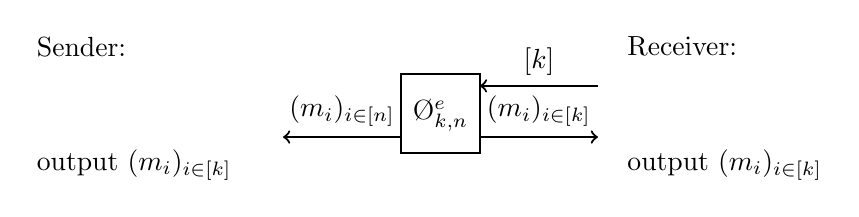
\begin{tikzpicture}
\node [anchor=west] at (0,5) {Sender:};
\node [anchor=west] at (7.5,5) {Receiver:};
\draw [thick] (4.75,4.65)--(5.75,4.65)--(5.75,3.65)--(4.75,3.65)--cycle;
\node at (5.25,4.125){$\O^{e}_{k,n}$};
\draw [thick, <-] (5.75,4.5)-- node [midway,above]{$[k]$}(7.25,4.5);
\draw [thick, ->] (5.75,3.85)-- node [midway,above]{$(m_i)_{i\in [k]}$}(7.25,3.85);
\draw [thick, <-] (3.25,3.85)-- node [midway,above]{$(m_i)_{i\in [n]}$}(4.75,3.85);
\node [anchor=west] at (0,3.5) {output $(m_i)_{i\in[k]}$};
\node [anchor=west] at (7.5,3.5) {output $(m_i)_{i\in[k]}$};
\end{tikzpicture}
}
% 	\framebox{\begin{minipage}{0.95\linewidth}
% 			Input: The sender \send and receiver \rec have no input.
% 			\begin{enumerate}
% 				\item \label{step:coin_step1} \rec sends $\set:=[k]$ to $\O^{u}_{k,n}$ and receives $(s_i)_{i\in \set}$ in response. \send receives $(s_i)_{i\in [n]}$. 
% 				\item \label{step:coin_step2} Both parties output the bits of $(s_i)_{i\in [k]}$.
% 			\end{enumerate}
% 	\end{minipage}}
	\caption{Coin flipping Protocol $\Pi^{\coin}$ in the $\O^{u}_{k,n}$ hybrid. For all $i\in[n]$, $m_i$ is in $\bits^\ell$}
	\label{fig:coinFlip}
\end{figure}


\begin{lemma}
	$\Pi^{\textsf{coin}}$ of \figureref{fig:coinFlip} realizes an ideal coin flipping protocol with unconditional security  in the $\O^{u}_{k,n}$ hybrid  (\definitionref{def:ot}).
\end{lemma}
\begin{proof}
	Trivial.
\end{proof}


\begin{figure}[t]
\centering
\framebox{
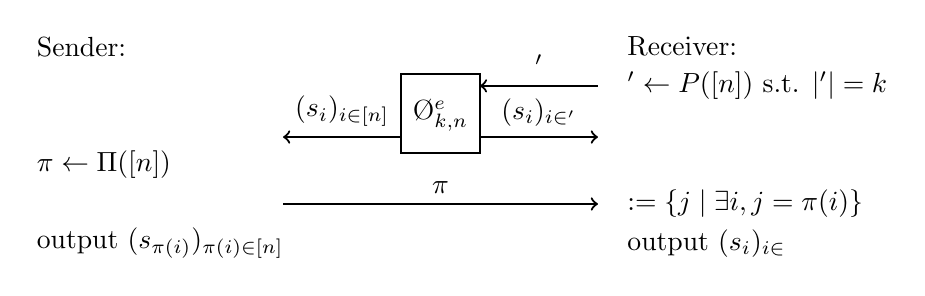
\begin{tikzpicture}
\node [anchor=west] at (0,5) {Sender:};
\node [anchor=west] at (7.5,5) {Receiver:};
\draw [thick] (4.75,4.65)--(5.75,4.65)--(5.75,3.65)--(4.75,3.65)--cycle;
\node at (5.25,4.125){$\O^{e}_{k,n}$};
\node [anchor=west] at (7.5,4.5){$\set'\gets \mathbb{P}([n])$ s.t. $|\set'|=k$};
\draw [thick, <-] (5.75,4.5)-- node [midway,above]{$\set'$}(7.25,4.5);
\draw [thick, ->] (5.75,3.85)-- node [midway,above]{$(s_i)_{i\in \set'}$}(7.25,3.85);
\node [anchor=west] at (0,3.5) {$\pi\leftarrow\Pi([n])$};
\draw [thick, ->] (3.25,3)-- node [midway, above]{$\pi$} (7.25,3);
\draw [thick, <-] (3.25,3.85)-- node [midway,above]{$(s_i)_{i\in [n]}$}(4.75,3.85);
\node [anchor=west] at (0,2.5) {output $(s_{\pi(i)})_{\pi(i)\in[n]}$};
\node [anchor=west] at (7.5,3) {$\set:=\{j \mid \exists i, j=\pi(i)\}$};
\node [anchor=west] at (7.5,2.5) {output $(s_i)_{i\in\set}$};
\end{tikzpicture}
}
% 	\framebox{\begin{minipage}{0.95\linewidth}
% 			Input: The sender \send and receiver \rec have no input.
% 			\begin{enumerate}
% 				\item \label{step:uniformSelect_step1} \rec uniformly samples $\set'\gets \mathbb{P}([n])$ s.t. $|\set'|=k$. \rec sends $\set'$ to $\OOT^{\E}$ and receives $(s_i')_{i\in \set'}$ in response. \send receives $(s_i')_{i\in [n]}$. 
% 				\item \label{step:uniformSelect_step2} \send samples a random permutation $\pi : [n] \rightarrow [n]$ and sends it to \rec.
% 				\item \label{step:uniformSelect_step3} \send outputs $(s_i)_{i\in [n]}$ and \rec outputs $(\set, (s_i)_{i\in\set})$ where $s_i:=s_{\pi(i)}'$ and $\set:=\{j \mid \exists i, j=\pi(i)\}$.
% 			\end{enumerate}
% 	\end{minipage}}
	\caption{Uniform Selection $k$-out-of-$n$ OT protocol $\Pi^{\E u}$ in the $\OOT^{\E}$ hybrid. $\Pi([n])$ is the set of permutations over $[n]$.}
	\label{fig:uniformSelect}
\end{figure}


\begin{lemma}
	$\Pi^{\E u}$ of \figureref{fig:uniformSelect} realizes the  Ideal Uniform Selection Endemic Message OT $\OOT^{\E u}$ (\definitionref{def:ot}) with unconditional security in the $\OOT^{\E}$ hybrid.
\end{lemma}


\begin{proof}
	\textcolor{red}{TODO}.
\end{proof}

\begin{remark}
	\textcolor{red}{Make some statement about how the sample transformation applies to the other OT message security notions.}
\end{remark}


\newcommand{\com}{\ensuremath{\mathsf{com}}\xspace}
\newcommand{\open}{\ensuremath{\mathsf{open}}\xspace}
\begin{figure}[t]
\centering
\framebox{
\begin{tikzpicture}
\node [anchor=west] at (0,5.5) {Sender:};
\node [anchor=west] at (7.5,5.5) {Receiver:};
\draw [thick] (4.75,4.65)--(5.75,4.65)--(5.75,3.65)--(4.75,3.65)--cycle;
\node at (5.25,4.125){$\O^{\rec}_{k,n}$};
\draw [thick, <-] (5.75,4.5)-- node [midway,above]{$\set,(s_i)_{i\in\set}$}(7.25,4.5);
\draw [thick, ->] (5.75,3.85)-- node [midway,above]{$(m_i)_{i\in \set'}$}(7.25,3.85);
\node [anchor=west] at (0,3.5) {$\forall i\in[n]$};
\node [anchor=west] at (0,3) {$\quad s_i:=H(s,m_i)$};
\draw [thick, ->] (3.25,5)-- node [midway, above]{$c:=\com(s)$} (7.25,5);
\draw [thick, ->] (3.25,3)-- node [midway, above]{$\open(c)$} (7.25,3);
\node [anchor=west] at (0,5) {$s\leftarrow\bits^\sec$};
\draw [thick, <-] (3.25,3.85)-- node [midway,above]{$(m_i)_{i\in [n]}$}(4.75,3.85);
\node [anchor=west] at (0,2) {output $(s_i)_{i\in[n]}$};
\node [anchor=west] at (7.5,2) {output $(s_i)_{i\in\set}$};
\node [anchor=west] at (7.5,3) {$\forall i\in\set$};
\node [anchor=west] at (7.5,2.5) {$\quad s_i:=H(s,m_i)$};
\end{tikzpicture}
}
% 	\framebox{\begin{minipage}{0.95\linewidth}
% 			Input: The sender \send and receiver \rec have no input.
% 			\begin{enumerate}
% 				\item \label{step:uniformSelect_step1} \rec uniformly samples $\set'\gets \mathbb{P}([n])$ s.t. $|\set'|=k$. \rec sends $\set'$ to $\OOT^{\E}$ and receives $(s_i')_{i\in \set'}$ in response. \send receives $(s_i')_{i\in [n]}$. 
% 				\item \label{step:uniformSelect_step2} \send samples a random permutation $\pi : [n] \rightarrow [n]$ and sends it to \rec.
% 				\item \label{step:uniformSelect_step3} \send outputs $(s_i)_{i\in [n]}$ and \rec outputs $(\set, (s_i)_{i\in\set})$ where $s_i:=s_{\pi(i)}'$ and $\set:=\{j \mid \exists i, j=\pi(i)\}$.
% 			\end{enumerate}
% 	\end{minipage}}
	\caption{Uniform $k$-out-of-$n$ OT protocol $\Pi^{\U}$ in the $\OOT^{\rec}$ hybrid and random oracle model.}
	\label{fig:uniformSelect}
\end{figure}

\begin{figure}[t!]
	\vspace{-1cm}
	\framebox{
	\begin{minipage}{0.95\linewidth}\small
			\textsc{Parameters:} $\kappa$ is the computational security parameter. $m$ denotes the number of OTs. $N$ denotes the number of messages each OT has. $\mathcal{C}$ is an $[\nc,\kc,\dc]$ binary linear code such that $\kc=\log_2 N$ and $\dc\geq \kappa$. A bijective map $map : [N]\rightarrow\mathbb{F}^\kc$.\\
			\textsc{Requirements:} $\H : [m] \times \mathbb{F}_2^\nc \rightarrow \mathbb{F}_2^\kappa$ is a random oracle.			
			Let $m'=m+s$ where $s$ is defined in \stepref{step:consistency}. \OOT is an 1-out-of-2 OT oracle with output messages in $\mathbb{F}_2^{m'}$.
			\\
			
			\textsc{Extend:} On input $(\textsc{Extend})$ from \send and $(\textsc{Extend}, (x_1,...,x_m)\in[N]^m)$ from \rec.
			\begin{enumerate}
				\item\label{step:extInit} Both parties invoke $\nc$  instances of $\OOT$  where \send takes the role of the receiver. If $\OOT$ has inputs, the corresponding party  locally samples them uniformly from the input domains. \send receives $(\bb'\in\{1,2\}^\nc, \{\tt^j_{b_j}\}_{j\in [\nc]})$ where $\bb_i=(\bb_i'-1)\in\{0,1\}$. \rec receives $\{(\tt^j_0,\tt^j_1)\}_{j\in [\nc]}$. Let $T_0\in \mathbb{F}^{m'\times \nc}_2$ denote the matrix formed by concatenating the column vectors $\tt^1_0||...||\tt^\nc_0$. \\
				
				%				\item \rec constructs matrices $T_0,T_1\in \mathbb{F}^{m'\times \nc}_2$ from the seeds $\{(\rr^j_0,\rr^j_1)\}_{j\in [\nc]}$ so that the respective columns are:
				%				$$
				%					\tt^j_0 := \PRG(\rr^j_0)\in \mathbb{F}^{m'}_2,\qquad \tt^j_1 := \PRG(\rr^j_1)\in \mathbb{F}^{m'}_2,\qquad \forall j\in[\nc]
				%				$$
				%				In the same way \send produces $\tt^j_{b_j}$, for each $j\in[\nc]$. Summarizing, \rec holds $\{(\tt^j_0,\tt^j_1)\}_{j\in[\nc]}$ and \send holds $\{\tt^j_{b_j}\}_{j\in[\nc]}$.
				%				
				\item\label{step:extSendU} \rec  defines $\ww_i:=map(x_i)$ for $i\in[m]$ and  samples random $\ww_{m+\ell}\gets \mathbb{F}^\kc_2$, for $\ell\in[s]$. Then constructs a matrix $C\in\mathbb{F}^{m'\times \nc}_2$ such that each row $\cc_i$ is the codeword $\mathcal{C}(\ww_i)$. Then, \rec sends to \send the values
				$$
				\uu^j :=\tt^j_0 +\tt^j_1+\cc^j, \qquad \forall j\in[\nc],
				$$
				where $\cc^j$ is the $j$-th column of $C$.
				
				\item\label{step:extCompQ} \send receives $\uu^j\in\mathbb{F}^{m'}_2$ and computes
				$$
				\qq^j := b_j \cdot \uu^j +\tt^j_{b_j} = b_j\cdot \cc^j+\tt^j_0,\qquad \forall j\in[\nc]
				$$
				that form the columns of an $(m'\times \nc)$ matrix $Q$. Denoting the rows of $T_0, Q$ by $\tt_i,\qq_i$, \rec now holds $\cc_i,\tt_i$ and \send holds $\bb, \qq_i$ so that 
				$$
				\qq_i = \cc_i\odot \bb+\tt_i,\qquad \forall i\in[m'].
				$$
				
				\item \emph{Consistency check:}\label{step:consistency} \rec  proves in zero knowledge that given their view:
				\begin{center}
					$	\forall i\in[m], \exists w\in\mathbb{F}^\kc_2\  s.t.\  \cc_i \text{ decodes to } w \quad  \text{and}$ \\
					$\forall w'\in\mathbb{F}^\kc_2\setminus\{w\},$ the distribution of \\
					$(\cc_i+\mathcal{C}(w))\odot \bb$\\      
					has at least $\log_2(1/\negl)$ bits of entropy.
				\end{center}
				
				 For example, the proof of \cite{C:KelOrsSch15} for $N=2$ or \cite{RSA:OrrOrsSch17} otherwise. $s\geq0$ is specified by the proof protocol.
%				\begin{itemize}
%					\item Both parties query the challenge oracle $\O^{\textsf{chllng}}$ on input $u^j$ for $j\in[\nc]$  which samples and returns $X=\{(x_1^{\ell}, ...,x_m^{\ell} )\in \mathbb{F}^m_2\}_{\ell\in[s]}$ % := H'(\uu^1|| ... || \uu^\nc).
%					to both parties.
%					
%					\item \rec computes and sends, for $\ell \in[s]$:
%					$$
%					\widehat \tt^{\ell} := \sum_{i\in[m]} \tt_i \cdot x_i^\ell + \tt_{m+\ell}, \qquad \widehat \ww^\ell := \sum_{i\in[m]} \ww_i \cdot x_i^\ell + \ww_{m+\ell}
%					$$
%					
%					\item \send computes $\widehat \qq^\ell := \sum_{i\in[m]} \qq_i \cdot x^\ell_i + \qq_{m+\ell}$, and checks that:
%					$$
%					\widehat\tt^\ell + \widehat\qq^\ell = \mathcal{C}(\widehat\ww^\ell) \odot \bb, \qquad \forall\ell\in[s].
%					$$
%					If the check fails, \send sends $\textsf{Abort}$, and otherwise continues.
%				\end{itemize}
				\item \rec outputs $\vv_{i, x_j}:=\H(i,\tt_i)$ for all $i\in[m]$.
			\end{enumerate}
			
			
			\textsc{Output:} On input $(\textsc{Output}, (i,x))$ from \send. If $i\in[m],j\in[N]$, then \send outputs $\vv_{i,x}:=\H(i,\qq_i+\mathcal{C}(map(x))\odot \bb)$.
	\end{minipage}
	}
	\caption{ 1-out-of-$N$ OT Extension.}
	\label{fig:otExt}
\end{figure}
